\documentclass[12pt, a4paper]{article}

% ─── Pacchetti ──────────────────────────────────────────────────────────────
\usepackage[utf8]{inputenc}
\usepackage[T1]{fontenc}
\usepackage[italian]{babel}
\usepackage{geometry}
\usepackage{graphicx}
\usepackage{booktabs}
\usepackage{array}
\usepackage{longtable}
\usepackage{tabularx}
\usepackage{hyperref}
\usepackage{titlesec}
\usepackage{enumitem}
\usepackage{xcolor}
\usepackage{fancyhdr}
\usepackage{lastpage}
\usepackage{parskip}
\usepackage{microtype}
\usepackage{listings}
\usepackage{float}

\geometry{
  top=2.5cm,
  bottom=2.5cm,
  left=3cm,
  right=3cm
}

% ─── Colori ─────────────────────────────────────────────────────────────────
\definecolor{trentoBlue}{RGB}{0, 82, 147}
\definecolor{lightGray}{RGB}{245, 245, 245}
\definecolor{darkGray}{RGB}{80, 80, 80}

% ─── Intestazione e piè di pagina ───────────────────────────────────────────
\pagestyle{fancy}
\fancyhf{}
\fancyhead[L]{\small\textcolor{darkGray}{IoSonoTrento Analisi e Progettazione}}
\fancyhead[R]{\small\textcolor{darkGray}{D3 V1.0}}
\fancyfoot[C]{\small\thepage\ / \pageref{LastPage}}
\renewcommand{\headrulewidth}{0.4pt}

% ─── Titoli delle sezioni ───────────────────────────────────────────────────
\titleformat{\section}
  {\large\bfseries\color{trentoBlue}}
  {\thesection.}{0.5em}{}[\titlerule]

\titleformat{\subsection}
  {\normalsize\bfseries\color{trentoBlue}}
  {\thesubsection.}{0.5em}{}

\titleformat{\subsubsection}
  {\normalsize\bfseries}
  {\thesubsubsection.}{0.5em}{}

% ─── Hyperlink ──────────────────────────────────────────────────────────────
\hypersetup{
  colorlinks=true,
  linkcolor=trentoBlue,
  urlcolor=trentoBlue,
  pdftitle={IoSonoTrento - Analisi e Progettazione},
  pdfauthor={Team IoSonoTrento},
}

% ─── Comandi custom ─────────────────────────────────────────────────────────
\newcommand{\cmp}[1]{\textbf{CMP#1}}
\newcommand{\interfacciarichiesta}[1]{\textbf{Interfaccia richiesta #1:}}
\newcommand{\interfacciafornita}[1]{\textbf{Interfaccia fornita #1:}}

% ════════════════════════════════════════════════════════════════════════════
\begin{document}

% ─── Frontespizio ───────────────────────────────────────────────────────────
\thispagestyle{empty}

\begin{center}
  \vspace*{1cm}

  {\large Dipartimento di Ingegneria e Scienza dell'Informazione}

  \vspace{2cm}

  \textbf{Progetto:}\\[0.3cm]
  {\LARGE \textbf{IoSonoTrento}}

  \vspace{1cm}

  \textbf{Titolo del documento:}\\[0.3cm]
  {\Large \textbf{Analisi e Progettazione}}

  \vspace{2cm}

  \begin{tabular}{|>{\bfseries}p{3.5cm}|p{5cm}|>{\bfseries}p{3cm}|p{2.5cm}|}
    \hline
    Doc. Name & \textit{D3-IoSonoTrentoAnalisiProgettazione} & Doc. Number & D3 V1.0 \\
    \hline
    Description & Documento di design & & \\
    \hline
  \end{tabular}

  \vspace{3cm}

  {\small
    \begin{tabular}{ll}
      \textbf{Corso:}  & Ingegneria del Software \\
      \textbf{Anno Accademico:} & 2025/2026 \\
    \end{tabular}
  }
\end{center}

\newpage

% ─── Indice ─────────────────────────────────────────────────────────────────
\tableofcontents
\newpage

% ════════════════════════════════════════════════════════════════════════════
\section*{Scopo del documento}
\addcontentsline{toc}{section}{Scopo del documento}

Il presente documento riporta il design del progetto \textbf{IoSonoTrento} piattaforma
di partecipazione civica per il Comune di Trento attraverso l'utilizzo di un diagramma dei
componenti e di un diagramma delle classi. Partendo dall'analisi dei requisiti e dagli use-case
individuati nelle fasi precedenti, vengono qui formalizzati i componenti architetturali del sistema,
le loro interfacce, e la struttura delle classi del dominio, con lo scopo di guidare l'implementazione
backend e frontend dell'applicazione.

% ════════════════════════════════════════════════════════════════════════════
\section{Analisi dei Componenti}

% ────────────────────────────────────────────────────────────────────────────
\subsection{Definizione dei componenti}

In questa sezione vengono descritti i componenti con le apposite interfacce previste per il software
\textbf{IoSonoTrento}.

% ····················································
\subsubsection*{CMP1: Gestione autenticazione}
\addcontentsline{toc}{subsubsection}{CMP1: Gestione autenticazione}

\textbf{Descrizione:}\\
Il componente si occupa dell'autenticazione degli utenti del sistema, che si divide in due percorsi
distinti in base al ruolo. I \textit{Cittadini} accedono esclusivamente tramite Google OAuth 2.0
(Single Sign-On): il sistema li reindirizza ai server Google, riceve il token di autorizzazione e,
al primo accesso, obbliga il cittadino a completare il proprio profilo prima di emettere un JWT.
Gli \textit{Operatori} accedono tramite credenziali username/password; il sistema verifica le
credenziali, confronta la password con l'hash bcrypt salvato e rilascia un JWT di sessione.

\interfacciarichiesta{credenziali operatore}\\
Username e password dell'operatore, forniti tramite il form di login. La password viene confrontata
con il digest bcrypt memorizzato nel database.

\interfacciarichiesta{autorizzazione OAuth da Google}\\
Token OAuth 2.0 ottenuto al termine del flusso Google SSO. Il componente verifica l'autenticità del
token, estrae l'e-mail e l'ID Google del cittadino e crea (o recupera) il profilo corrispondente.

\interfacciafornita{richiesta OAuth verso Google}\\
Reindirizzamento del browser del cittadino verso il server di autorizzazione Google
(\texttt{/auth/google}), con i parametri \texttt{client\_id}, \texttt{scope} e
\texttt{redirect\_uri}.

\interfacciafornita{JWT di sessione}\\
Token JWT firmato con il \texttt{JWT\_SECRET}, contenente l'identificativo dell'utente e il suo
ruolo (\texttt{operatore} o \texttt{cittadino}). Viene incluso nelle successive richieste come
header \texttt{Authorization: Bearer <token>}.

\interfacciarichiesta{completamento profilo cittadino}\\
Al primo accesso Google, se \texttt{profiloCompleto = false}, il cittadino deve fornire data di
nascita, circoscrizione di residenza, categoria occupazionale e genere tramite
\texttt{POST /auth/complete-profile}. Nome ed e-mail sono invece importati automaticamente dal
profilo Google.

\interfacciafornita{autenticazione}\\
Permette all'utente autenticato di accedere a tutte le funzionalità a lui riservate, garantendo
l'accesso sicuro alle risorse protette tramite il middleware \texttt{protect}.

% ····················································
\subsubsection*{CMP2: Gestione database}
\addcontentsline{toc}{subsubsection}{CMP2: Gestione database}

\textbf{Descrizione:}\\
Il componente funge da strato di persistenza del sistema. Gestisce la connessione al database
MongoDB e mette a disposizione degli altri componenti le operazioni CRUD sulle entità del dominio
(\textit{Cittadino}, \textit{Operatore}, \textit{Consultazione}, \textit{Domanda},
\textit{Iniziativa}, \textit{RispostaConsultazione}, \textit{VotoIniziativa}, \textit{Categoria},
\textit{Notifica}).
Applica la validazione degli schemi Mongoose prima di ogni scrittura.

\interfacciarichiesta{dati di registrazione operatore}\\
Username, password in chiaro, nome e cognome. Il componente salva la password come hash bcrypt e
imposta \texttt{isRoot} a \texttt{false}: l'unico operatore \textit{root} è quello creato dal seed
iniziale.

\interfacciarichiesta{dati profilo cittadino}\\
Dati del cittadino (data di nascita, circoscrizione, genere, categoria occupazionale) necessari per
portare \texttt{profiloCompleto} a \texttt{true}; nome e cognome, importati da Google, sono
aggiornabili separatamente.

\interfacciarichiesta{dati consultazione}\\
Tipo (\texttt{votazione} | \texttt{sondaggio}), titolo, descrizione, date di inizio, fine e
discussione, domande associate, stato iniziale (\texttt{bozza}).

\interfacciarichiesta{risposta a consultazione}\\
Identificativo cittadino, identificativo consultazione, opzioni selezionate o testo libero. Viene
verificato che il cittadino non abbia già risposto alla stessa consultazione.

\interfacciarichiesta{dati iniziativa}\\
Titolo, descrizione, categoria, identificativo del cittadino proponente e stato iniziale
(\texttt{in\_attesa}).

\interfacciafornita{entità recuperate}\\
Oggetti JSON restituiti ai componenti che ne fanno richiesta (liste paginate, singoli documenti,
aggregazioni statistiche).

\interfacciafornita{modifiche al database}\\
Conferma delle operazioni di creazione, aggiornamento o eliminazione dei documenti.

% ····················································
\subsubsection*{CMP3: Gestione consultazioni}
\addcontentsline{toc}{subsubsection}{CMP3: Gestione consultazioni}

\textbf{Descrizione:}\\
Il componente si occupa del ciclo di vita delle consultazioni pubbliche, che comprendono sia le
\textit{votazioni} (con una singola domanda a risposta singola o multipla) sia i \textit{sondaggi}
(con più domande). Gli operatori creano le consultazioni in stato \texttt{bozza} e le pubblicano;
una volta pubblicate diventano votabili a partire dalla \texttt{data\_inizio}. Lo scheduler
(\textit{CMP7}) attiva automaticamente le bozze la cui \texttt{data\_inizio} è trascorsa e porta a
\texttt{concluso} le consultazioni alla \texttt{data\_fine}. I cittadini possono rispondere alle
consultazioni attive; l'operatore può infine archiviare quelle concluse.

\interfacciarichiesta{autenticazione}\\
JWT valido per distinguere il ruolo: solo gli operatori possono creare/modificare consultazioni;
i cittadini possono solo leggerle e rispondere.

\interfacciarichiesta{dati nuova consultazione}\\
Tipo, titolo, date, domande (una per votazione, array per sondaggio) e lo stato iniziale.

\interfacciarichiesta{risposta del cittadino}\\
Identificativo cittadino, identificativo consultazione e opzioni selezionate.

\interfacciafornita{lista consultazioni}\\
Elenco filtrato per tipo e/o stato, con paginazione e ordinamento per data.

\interfacciafornita{dettaglio consultazione}\\
Singolo documento con le domande associate e i metadati (stato, date, autore).

\interfacciafornita{conferma risposta registrata}\\
Esito positivo o negativo della registrazione della risposta del cittadino.

\interfacciafornita{statistiche votazione}\\
Aggregazione del numero di voti per opzione, con le relative percentuali, disponibile a qualunque
utente autenticato. Le aggregazioni demografiche dei votanti sono invece riservate agli operatori
(si veda \textit{CMP6}).

% ····················································
\subsubsection*{CMP4: Gestione iniziative}
\addcontentsline{toc}{subsubsection}{CMP4: Gestione iniziative}

\textbf{Descrizione:}\\
Il componente gestisce le iniziative civiche proposte dai cittadini. Un cittadino può creare
un'iniziativa fornendo titolo, descrizione e categoria; gli altri cittadini possono sostenerla con
un voto. Gli operatori moderano le iniziative, portandole dallo stato \texttt{in\_attesa} a
\texttt{approvata} o \texttt{rifiutata} con una motivazione. Al termine della moderazione, il
componente delega a \textit{CMP8} la creazione della notifica per il cittadino proponente.

\interfacciarichiesta{autenticazione}\\
JWT valido; il componente verifica il ruolo per decidere quali operazioni sono consentite.

\interfacciarichiesta{dati nuova iniziativa}\\
Titolo, descrizione, identificativo categoria. L'identificativo del cittadino viene estratto dal JWT.

\interfacciarichiesta{decisione di moderazione}\\
Nuovo stato (\texttt{approvata} | \texttt{rifiutata}) e motivazione testuale, forniti
dall'operatore tramite \texttt{PATCH /iniziative/:id/modera}.

\interfacciafornita{lista iniziative}\\
Elenco delle iniziative, filtrabile per stato e categoria, con il numero di voti ricevuti.

\interfacciafornita{dettaglio iniziativa}\\
Documento con tutti i metadati e la descrizione completa, arricchito come la lista con il nome
della categoria, il nominativo del cittadino proponente e il numero di voti ricevuti; per i
cittadini include il flag \texttt{ha\_votato}.

\interfacciafornita{esito voto iniziativa}\\
Conferma dell'aggiunta o rimozione del voto di supporto di un cittadino a un'iniziativa.

% ····················································
\subsubsection*{CMP5: Gestione profilo cittadino}
\addcontentsline{toc}{subsubsection}{CMP5: Gestione profilo cittadino}

\textbf{Descrizione:}\\
Il componente raggruppa le funzionalità legate al profilo del cittadino: la visualizzazione dei
propri dati, il completamento del profilo al primo accesso, la modifica dei dati anagrafici e il
logout. Per gli operatori espone funzionalità analoghe: visualizzazione del profilo, cambio
password e promozione a \textit{root}.

\interfacciarichiesta{autenticazione}\\
JWT valido per garantire che ogni utente acceda solo al proprio profilo.

\interfacciarichiesta{dati completamento profilo}\\
Data di nascita, circoscrizione, categoria occupazionale e genere forniti dal cittadino tramite
\texttt{POST /auth/complete-profile}.

\interfacciarichiesta{dati aggiornamento anagrafica}\\
Nome e cognome aggiornati, inviati dal cittadino tramite \texttt{PATCH /cittadino/me}.

\interfacciarichiesta{nuova password operatore}\\
Password attuale e nuova password, utilizzate per il cambio credenziali
(\texttt{PATCH /operatore/me/password}).

\interfacciafornita{profilo utente}\\
Dati anagrafici e metadati dell'account (data di registrazione, stato \texttt{loggedIn},
\texttt{profiloCompleto}).

\interfacciafornita{conferma logout}\\
Aggiornamento del flag \texttt{loggedIn} a \texttt{false} e risposta di conferma al client.

% ····················································
\subsubsection*{CMP6: Gestione statistiche}
\addcontentsline{toc}{subsubsection}{CMP6: Gestione statistiche}

\textbf{Descrizione:}\\
Il componente aggrega i dati di partecipazione alle consultazioni per produrre statistiche
visualizzabili dagli operatori. Il \textit{riepilogo sintetico} calcola, per ogni opzione, il numero
di voti ricevuti e la percentuale sul totale dei votanti. Il \textit{riepilogo demografico} incrocia
i voti con i dati del cittadino votante e produce la distribuzione per genere, per fascia d'età
(derivata dalla \texttt{dataNascita}: 18--25, 26--35, 36--50, oltre 50), per categoria occupazionale
e l'andamento giornaliero della partecipazione. Espone queste aggregazioni tramite le API di
reportistica.

\interfacciarichiesta{dati risposte}\\
Insieme delle \textit{RispostaConsultazione} associate a una consultazione, con gli identificativi
dei cittadini rispondenti.

\interfacciarichiesta{dati anagrafici cittadini}\\
Dati dei cittadini, recuperati tramite \textit{join} sulla collezione \textit{Cittadino} nel momento
in cui la statistica viene richiesta.

\interfacciafornita{statistiche aggregate}\\
JSON con il conteggio voti per opzione e le distribuzioni per aggregazioni.

% ····················································
\subsubsection*{CMP7: Scheduler consultazioni}
\addcontentsline{toc}{subsubsection}{CMP7: Scheduler consultazioni}

\textbf{Descrizione:}\\
Il componente implementa un job schedulato (via \texttt{node-cron}, esecuzione oraria) che
gestisce le transizioni automatiche di stato delle consultazioni. All'avvio dell'applicazione
esegue immediatamente un ciclo di controllo. Le transizioni gestite sono:
$\texttt{bozza} \to \texttt{attivo}$ quando \texttt{data\_inizio} è trascorsa e
$\texttt{attivo} \to \texttt{concluso}$ quando \texttt{data\_fine} è trascorsa. Le sole transizioni
non automatiche sono l'archiviazione ($\texttt{concluso} \to \texttt{archiviato}$) e la
pubblicazione anticipata di una bozza, entrambe a carico dell'operatore.

\interfacciarichiesta{lista consultazioni attive/in bozza}\\
Interrogazione periodica al database per recuperare le consultazioni in stato \texttt{bozza} o
\texttt{attivo} che soddisfano i criteri di transizione.

\interfacciafornita{aggiornamento stato consultazione}\\
Scrittura del nuovo stato nel database.

% ····················································
\subsubsection*{CMP8: Sistema di notifiche}
\addcontentsline{toc}{subsubsection}{CMP8: Sistema di notifiche}

\textbf{Descrizione:}\\
Il componente gestisce le notifiche in-app destinate ai cittadini. Attualmente le notifiche vengono
generate automaticamente dal componente \textit{CMP4 Gestione Iniziative} al termine della
moderazione: il cittadino proponente riceve una notifica quando la propria iniziativa viene
\texttt{approvata} o \texttt{rifiutata}. Il componente espone API per recuperare le notifiche,
segnarle come lette singolarmente o tutte insieme. Il frontend effettua polling ogni 2 minuti
per aggiornare il contatore delle notifiche non lette nella topbar.

\interfacciarichiesta{evento di moderazione}\\
Segnale proveniente da \textit{CMP4} al termine della \texttt{PATCH /iniziative/:id/modera}:
contiene lo stato assegnato (\texttt{approvata} | \texttt{rifiutata}), la motivazione e
l'identificativo del cittadino destinatario.

\interfacciarichiesta{autenticazione}\\
JWT valido con ruolo \texttt{cittadino}; ogni cittadino può leggere e gestire solo le proprie
notifiche.

\interfacciafornita{lista notifiche}\\
Elenco delle notifiche del cittadino autenticato, ordinate dalla più recente, con il campo
\texttt{letta} per distinguere le notifiche nuove da quelle già viste
(\texttt{GET /notifiche}).

\interfacciafornita{conferma lettura}\\
Aggiornamento del flag \texttt{letta} a \texttt{true} per una singola notifica
(\texttt{PATCH /notifiche/:id/letta}) o per tutte quelle non lette
(\texttt{PATCH /notifiche/leggi-tutte}).

% ────────────────────────────────────────────────────────────────────────────
\subsection{Diagramma dei componenti}

Viene riportato di seguito il diagramma complessivo di tutti i componenti di sistema e le loro
interconnessioni descritte in precedenza.

\begin{figure}[H]
  \centering
      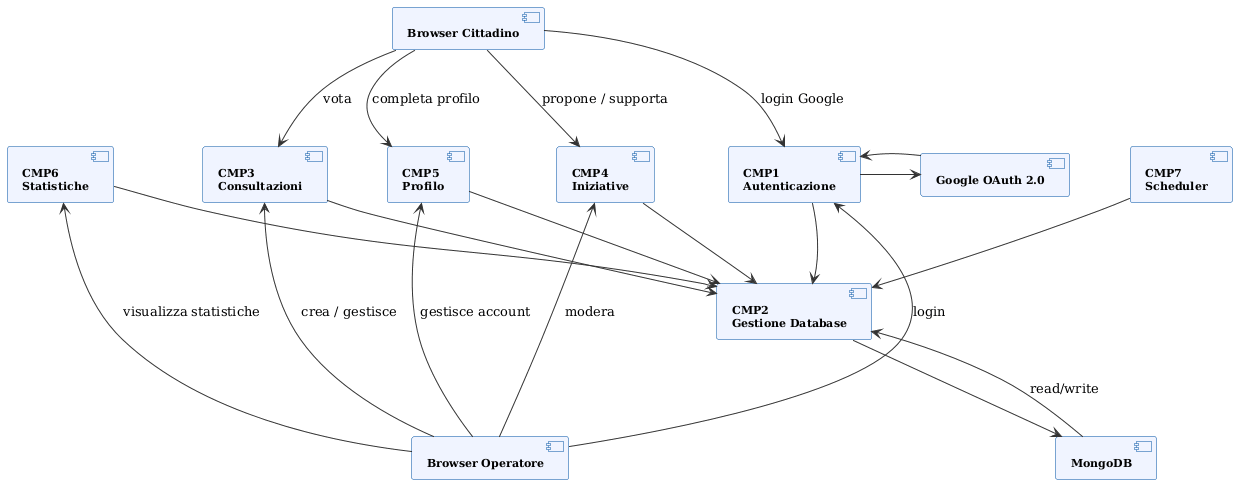
\includegraphics[width=\textwidth]{diagrams/ComponentDiagram.png}
  \caption{Diagramma dei componenti IoSonoTrento}
  \label{fig:diagramma-componenti}
\end{figure}

% ════════════════════════════════════════════════════════════════════════════
\section{Diagramma delle classi}

Nel presente capitolo vengono presentate le classi previste nell'ambito del progetto
\textbf{IoSonoTrento}. Ogni componente presentato nel capitolo precedente si riflette in una o
più classi del dominio. Tutte le classi sono caratterizzate da: un nome, una lista di attributi
che identificano i dati gestiti, e una lista di metodi che definiscono le operazioni previste.
In questo processo si è proceduto a massimizzare la coesione e minimizzare l'accoppiamento tra
classi.

% ────────────────────────────────────────────────────────────────────────────
\subsection*{1. Cittadino}
\addcontentsline{toc}{subsection}{1. Cittadino}

Il \textit{Cittadino} è l'utente finale della piattaforma. Accede tramite Google OAuth, può
partecipare a consultazioni, proporre e votare iniziative. Al primo accesso il suo profilo è
incompleto (\texttt{profiloCompleto = false}) e deve essere completato prima di poter operare.

\begin{figure}[H]
  \centering
      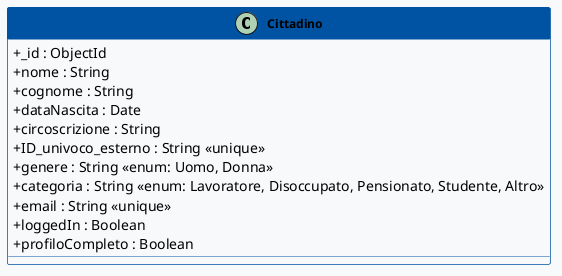
\includegraphics[width=\textwidth]{diagrams/Cittadino.png}
  \caption{Classe Cittadino}
\end{figure}

\noindent\textbf{Attributi principali:}
\begin{itemize}
  \item \texttt{\_id}: ObjectId univoco MongoDB
  \item \texttt{nome}, \texttt{cognome}: dati anagrafici
  \item \texttt{email}: indirizzo e-mail Google
  \item \texttt{ID\_univoco\_esterno}: Google ID (sub claim del token OAuth)
  \item \texttt{dataNascita}: data di nascita (usata per le statistiche per fascia d'età)
  \item \texttt{circoscrizione}: circoscrizione di residenza
  \item \texttt{genere}: \texttt{Uomo} | \texttt{Donna} (usato per le statistiche demografiche)
  \item \texttt{categoria}: categoria occupazionale (\texttt{Lavoratore}, \texttt{Disoccupato},
        \texttt{Pensionato}, \texttt{Studente}, \texttt{Altro})
  \item \texttt{profiloCompleto}: booleano, \texttt{false} al primo accesso
  \item \texttt{loggedIn}: booleano, aggiornato a ogni login/logout
\end{itemize}

\noindent\textbf{Metodi principali:}
\begin{itemize}
  \item \texttt{completeProfile(dati)}: imposta \texttt{dataNascita}, \texttt{circoscrizione},
        \texttt{genere} e \texttt{categoria}; porta \texttt{profiloCompleto} a \texttt{true}
  \item \texttt{updateProfile(dati)}: aggiorna \texttt{nome} e \texttt{cognome}
  \item \texttt{logout()}: aggiorna \texttt{loggedIn} a \texttt{false}
  \item \texttt{getProfile()}: restituisce i dati del profilo
\end{itemize}

% ────────────────────────────────────────────────────────────────────────────
\subsection*{2. Operatore}
\addcontentsline{toc}{subsection}{2. Operatore}

L'\textit{Operatore} è il dipendente comunale che gestisce la piattaforma: crea consultazioni,
modera le iniziative, gestisce gli altri operatori. L'operatore \textit{root} (creato dal seed
iniziale) può promuovere altri operatori.

\begin{figure}[H]
  \centering
      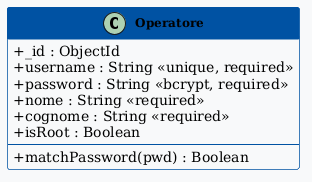
\includegraphics[width=\textwidth]{diagrams/Operatore.png}
  \caption{Classe Operatore}
\end{figure}

\noindent\textbf{Attributi principali:}
\begin{itemize}
  \item \texttt{\_id}: ObjectId univoco MongoDB
  \item \texttt{username}: identificativo di accesso univoco
  \item \texttt{password}: hash bcrypt della password
  \item \texttt{nome}, \texttt{cognome}: dati anagrafici del dipendente comunale
  \item \texttt{isRoot}: booleano, consente la gestione degli altri operatori
\end{itemize}

\noindent\textbf{Metodi principali:}
\begin{itemize}
  \item \texttt{login(username, password)}: verifica le credenziali e rilascia un JWT
  \item \texttt{changePassword(vecchiaPassword, nuovaPassword)}: aggiorna l'hash bcrypt
  \item \texttt{promote(operatoreId)}: promuove un operatore (solo per isRoot)
  \item \texttt{register(username, password, nome, cognome)}: crea un nuovo account operatore
        (solo per isRoot); il nuovo account ha sempre \texttt{isRoot = false}
  \item \texttt{getProfile()}: restituisce le informazioni dell'operatore.
\end{itemize}

% ────────────────────────────────────────────────────────────────────────────
\subsection*{3. Consultazione}
\addcontentsline{toc}{subsection}{3. Consultazione}

La \textit{Consultazione} rappresenta il fulcro della partecipazione civica. Utilizza un pattern
discriminato di Mongoose: se il tipo è \texttt{votazione}, ha una singola domanda
(\texttt{ID\_domanda}); se è \texttt{sondaggio}, ha un array di domande
(\texttt{ID\_domande[]}). Questi due campi sono mutuamente esclusivi.
Lo stato \texttt{concluso} viene impostato automaticamente dal sistema 
allo scadere di \texttt{data\_fine}, senza intervento dell'operatore.

\begin{figure}[H]
  \centering
      % doesnt render wtf%
      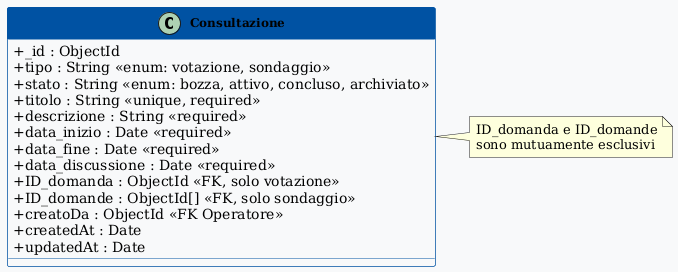
\includegraphics[width=\textwidth]{diagrams/Consultazione.png}
  \caption{Classe Consultazione}
\end{figure}

\noindent\textbf{Attributi principali:}
\begin{itemize}
  \item \texttt{tipo}: \texttt{votazione} | \texttt{sondaggio}
  \item \texttt{titolo}: titolo della consultazione (univoco)
  \item \texttt{descrizione}: testo descrittivo della consultazione
  \item \texttt{stato}: \texttt{bozza} $\to$ \texttt{attivo} $\to$ \texttt{concluso}
        $\to$ \texttt{archiviato}
  \item \texttt{data\_inizio}, \texttt{data\_fine}: intervallo temporale di attivazione
  \item \texttt{data\_discussione}: data della sessione pubblica di discussione
  \item \texttt{ID\_domanda}: riferimento alla domanda (solo votazione)
  \item \texttt{ID\_domande}: array di riferimenti alle domande (solo sondaggio)
  \item \texttt{creatoDa}: riferimento all'operatore creatore
\end{itemize}

\noindent\textbf{Metodi principali:}
\begin{itemize}
  \item  \texttt{update(modifiche)}: se in stato di bozza, permette di modificarne i campi ammessi. 
  \item \texttt{publish()}: porta lo stato da \texttt{bozza} ad \texttt{attivo}
  \item \texttt{conclude()}: porta lo stato da \texttt{attivo} a \texttt{concluso}
  \item \texttt{archive()}: porta lo stato da \texttt{concluso} ad \texttt{archiviato}
  \item \texttt{getStatistiche()}: aggrega e restituisce le statistiche di partecipazione
\end{itemize}

% ────────────────────────────────────────────────────────────────────────────
\subsection*{4. Domanda}
\addcontentsline{toc}{subsection}{4. Domanda}

La \textit{Domanda} è l'unità di quesito associabile a una consultazione. Supporta due
modalità: risposta singola (radio) e risposta multipla (checkbox).

\begin{figure}[H]
  \centering
      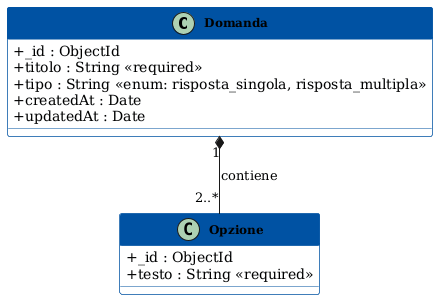
\includegraphics[width=\textwidth]{diagrams/Domanda.png}
  \caption{Classe Domanda}
\end{figure}

\noindent\textbf{Attributi principali:}
\begin{itemize}
  \item \texttt{titolo}: testo del quesito
  \item \texttt{opzioni}: array di sotto-documenti \texttt{Opzione}, ciascuno con un proprio
        \texttt{\_id} e il campo \texttt{testo}; ne servono almeno due. È l'\texttt{\_id}
        dell'opzione a essere referenziato dalle risposte dei cittadini
  \item \texttt{tipo}: \texttt{risposta\_singola} | \texttt{risposta\_multipla}
\end{itemize}

% ────────────────────────────────────────────────────────────────────────────
\subsection*{5. Iniziativa}
\addcontentsline{toc}{subsection}{5. Iniziativa}

L'\textit{Iniziativa} è la proposta civica che un cittadino può presentare alla municipalità.
Dopo la creazione è in attesa di moderazione da parte di un operatore.

\begin{figure}[H]
  \centering
      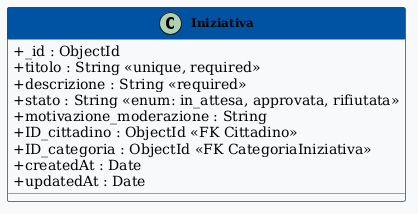
\includegraphics[width=\textwidth]{diagrams/Iniziativa.png}
  \caption{Classe Iniziativa}
\end{figure}

\noindent\textbf{Attributi principali:}
\begin{itemize}
  \item \texttt{titolo}: titolo dell'iniziativa
  \item \texttt{descrizione}: testo esteso della proposta
  \item \texttt{ID\_cittadino}: riferimento al cittadino proponente
  \item \texttt{ID\_categoria}: riferimento alla categoria tematica
  \item \texttt{stato}: \texttt{in\_attesa} | \texttt{approvata} | \texttt{rifiutata}
  \item \texttt{motivazione\_moderazione}: testo della motivazione dell'operatore
\end{itemize}

\noindent\textbf{Metodi principali:}
\begin{itemize}
  \item \texttt{modera(stato, motivazione)}: aggiorna lo stato e salva la motivazione
  \item \texttt{getVoti()}: restituisce il numero di voti di supporto ricevuti
\end{itemize}

% ────────────────────────────────────────────────────────────────────────────
\subsection*{6. RispostaConsultazione}
\addcontentsline{toc}{subsection}{6. RispostaConsultazione}

La \textit{RispostaConsultazione} è la classe di join tra \textit{Cittadino} e
\textit{Consultazione}. Registra le opzioni selezionate o le risposte testuali per ogni domanda
a cui il cittadino ha risposto.

\begin{figure}[H]
  \centering
      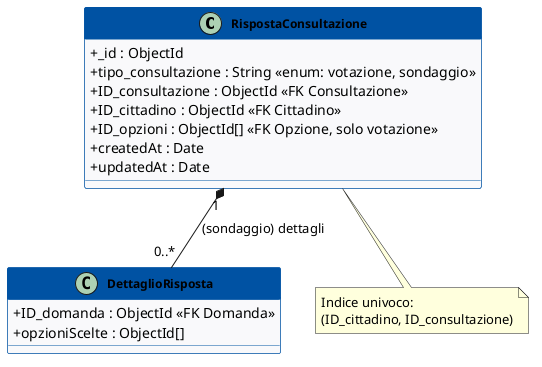
\includegraphics[width=\textwidth]{diagrams/RispostaConsultazione.png}
  \caption{Classe Risposta Consultazione}
\end{figure}

\noindent\textbf{Attributi principali:}
\begin{itemize}
  \item \texttt{ID\_cittadino}: riferimento al cittadino rispondente
  \item \texttt{ID\_consultazione}: riferimento alla consultazione
  \item \texttt{tipo\_consultazione}: \texttt{votazione} | \texttt{sondaggio}; determina quale dei
        due campi seguenti è valorizzato
  \item \texttt{ID\_opzioni}: array degli \texttt{\_id} delle opzioni scelte (solo votazione: un
        elemento per la risposta singola, più di uno per quella multipla)
  \item \texttt{dettagliRisposte}: array di coppie \texttt{ID\_domanda} $\to$
        \texttt{opzioniScelte[]} (solo sondaggio)
  \item \texttt{createdAt}, \texttt{updatedAt}: timestamp gestiti da Mongoose
\end{itemize}

\noindent Un indice univoco sulla coppia (\texttt{ID\_cittadino}, \texttt{ID\_consultazione})
garantisce a livello di database che un cittadino risponda una sola volta a una consultazione.

\noindent\textbf{Metodi principali:}
\begin{itemize}
  \item \texttt{esiste(cittadinoId,consultazioneId)}: controlla un eventuale risposta già presente 
\end{itemize}

% ────────────────────────────────────────────────────────────────────────────
\subsection*{7. VotoIniziativa}
\addcontentsline{toc}{subsection}{7. VotoIniziativa}

La \textit{VotoIniziativa} è la classe di join tra \textit{Cittadino} e \textit{Iniziativa}.
Registra il supporto espresso da un cittadino a un'iniziativa. Un cittadino può togliere il
proprio voto (\texttt{DELETE /cittadino/vote/iniziativa/:id}).

\begin{figure}[H]
  \centering
      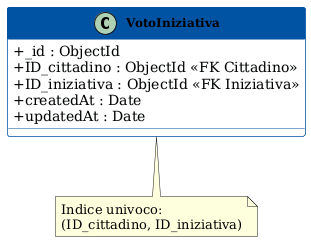
\includegraphics[width=\textwidth]{diagrams/VotoIniziativa.png}
  \caption{Classe Votto Iniziativa}
\end{figure}

\noindent\textbf{Attributi principali:}
\begin{itemize}
  \item \texttt{ID\_cittadino}: riferimento al cittadino votante
  \item \texttt{ID\_iniziativa}: riferimento all'iniziativa supportata
  \item \texttt{createdAt}, \texttt{updatedAt}: timestamp gestiti da Mongoose
\end{itemize}

\noindent Un indice univoco sulla coppia (\texttt{ID\_cittadino}, \texttt{ID\_iniziativa}) impedisce
a un cittadino di votare due volte la stessa iniziativa.

\noindent\textbf{Metodi principali:}
\begin{itemize}
  \item \texttt{esiste(cittadinoId,iniziativaId)}: controlla un eventuale risposta già presente 
\end{itemize}

% ────────────────────────────────────────────────────────────────────────────
\subsection*{8. Categoria Iniziativa}
\addcontentsline{toc}{subsection}{8. Categoria Iniziativa}

La \textit{Categoria Iniziativa} è una tassonomia tematica usata per classificare le iniziative (es.
\textit{Mobilità}, \textit{Ambiente}, \textit{Cultura}).

\begin{figure}[H]
  \centering
      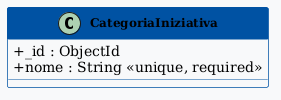
\includegraphics[width=\textwidth]{diagrams/CategoriaIniziativa.png}
  \caption{Classe Categoria Iniziativa}
\end{figure}

\noindent\textbf{Attributi principali:}
\begin{itemize}
  \item \texttt{nome}: nome della categoria (univoco)
\end{itemize}

% ────────────────────────────────────────────────────────────────────────────
\subsection*{9. Notifica}
\addcontentsline{toc}{subsection}{9. Notifica}

La \textit{Notifica} rappresenta un messaggio in-app generato automaticamente dal sistema e
destinato a un cittadino. Attualmente viene creata alla moderazione di un'iniziativa per
informare il proponente dell'esito (\texttt{approvata} o \texttt{rifiutata}).

\begin{figure}[H]
  \centering
      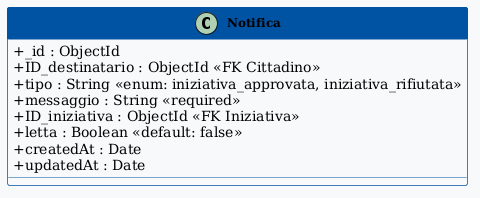
\includegraphics[width=0.7\textwidth]{diagrams/Notifica.png}
  \caption{Classe Notifica}
\end{figure}

\noindent\textbf{Attributi principali:}
\begin{itemize}
  \item \texttt{ID\_destinatario}: riferimento al cittadino destinatario
  \item \texttt{tipo}: \texttt{iniziativa\_approvata} | \texttt{iniziativa\_rifiutata}
  \item \texttt{messaggio}: testo della notifica generato automaticamente
  \item \texttt{ID\_iniziativa}: riferimento all'iniziativa a cui si riferisce la notifica
  \item \texttt{letta}: booleano, \texttt{false} alla creazione; portato a \texttt{true}
        quando il cittadino apre il pannello notifiche
\end{itemize}

\noindent\textbf{Metodi principali:}
\begin{itemize}
  \item \texttt{marcaLetta()}: imposta letta a true 
  \item \texttt{marcaTutteLette()}: marca come lette tutte le notifiche del destinatario che invoca il metodo. 
\end{itemize}

% ────────────────────────────────────────────────────────────────────────────
\subsection{Diagramma delle classi complessivo}

Viene riportato di seguito il diagramma delle classi complessivo che mostra le relazioni tra
tutte le classi del dominio.

\begin{figure}[H]
  \centering
      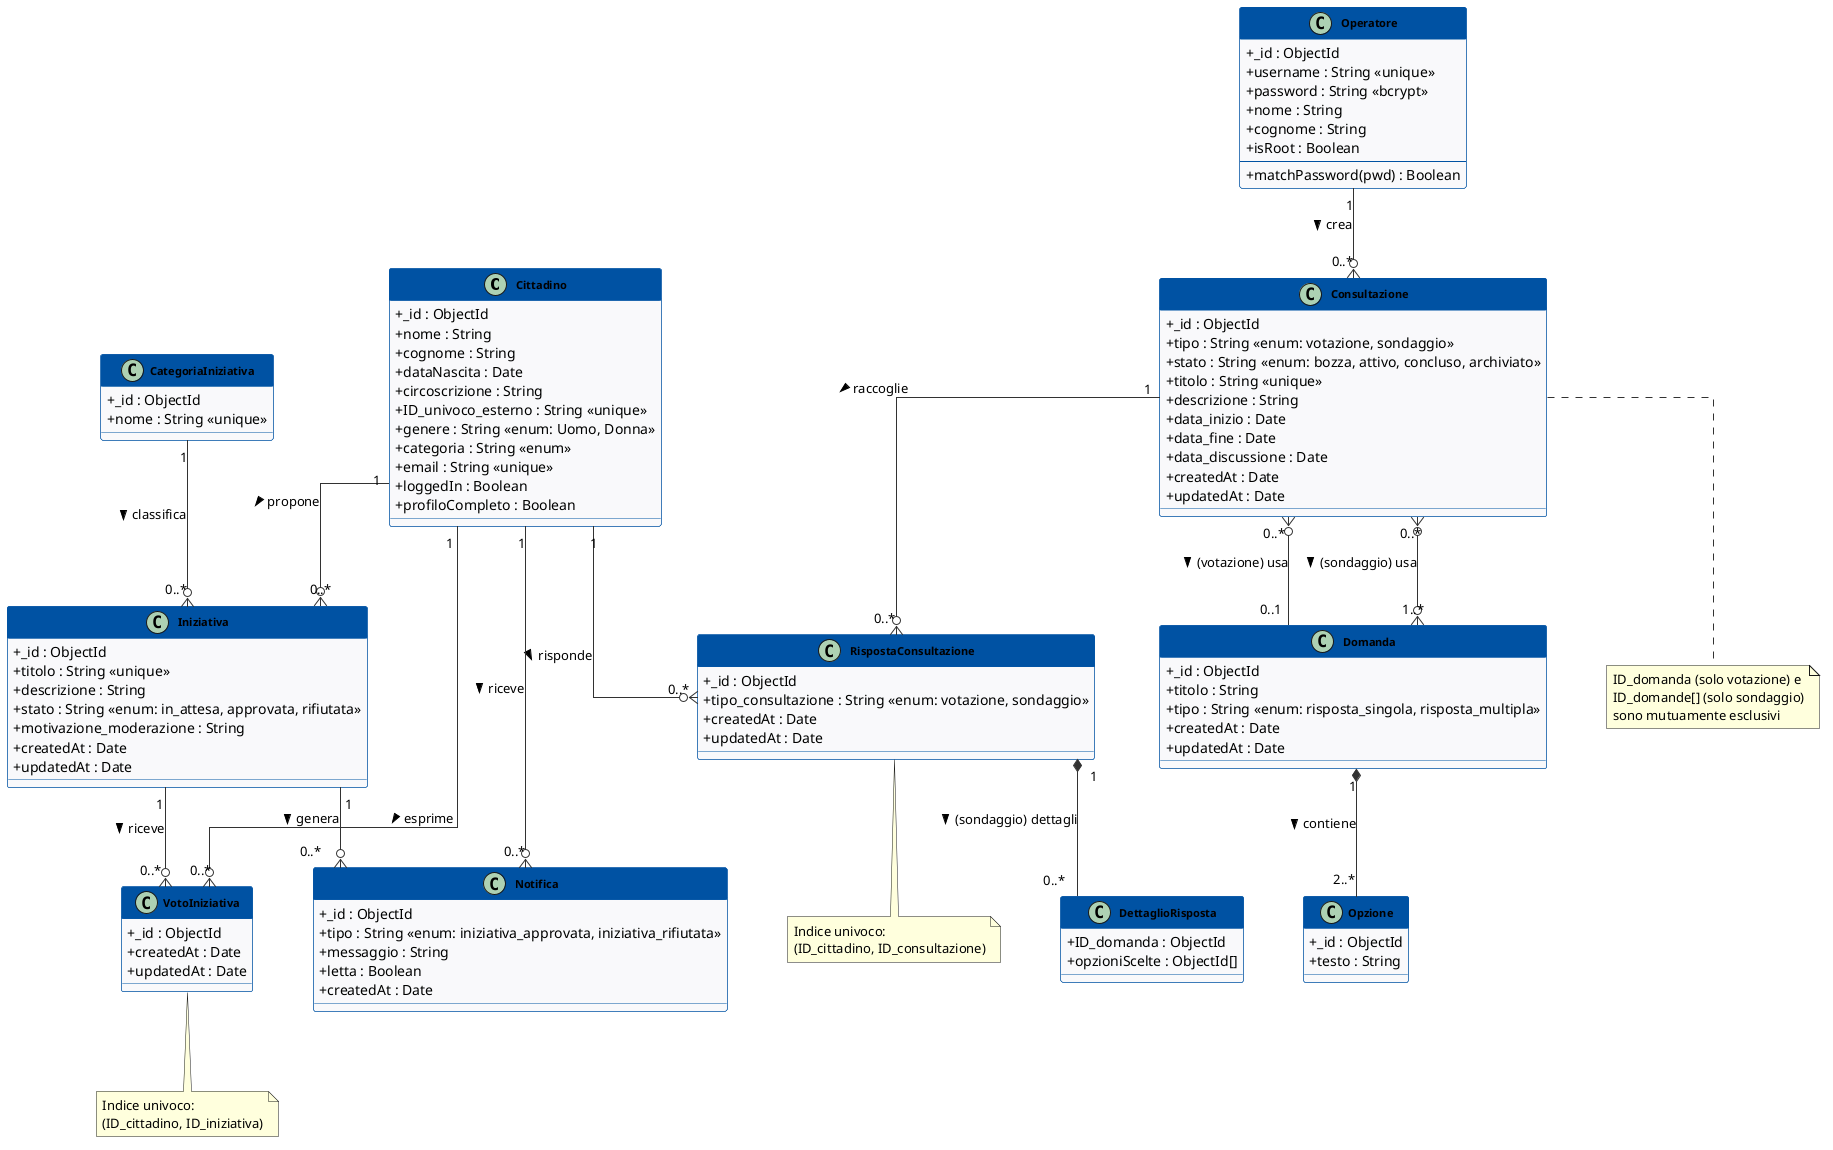
\includegraphics[width=\textwidth]{diagrams/ClassDiagramComplessivo.png}
  \caption{Diagramma delle classi complessivo IoSonoTrento}
  \label{fig:diagramma-classi}
\end{figure}

% ════════════════════════════════════════════════════════════════════════════
\section{Dal class diagram alle API}

Il diagramma delle classi delineato nella sezione precedente si traduce direttamente nelle API
REST esposte dal backend Node.js / Express. Ogni metodo delle classi corrisponde a uno o più
endpoint. Di seguito viene riportata la mappatura tra classi/metodi e route HTTP.

\vspace{0.5cm}

\begin{longtable}{>{\ttfamily\small}p{0.38\textwidth} p{0.14\textwidth} >{\ttfamily\small}p{0.38\textwidth}}
  \toprule
  \normalfont\textbf{Classe / Metodo} & \textbf{Metodo HTTP} & \normalfont\textbf{Endpoint} \\
  \midrule
  \endfirsthead
  \toprule
  \normalfont\textbf{Classe / Metodo} & \textbf{Metodo HTTP} & \normalfont\textbf{Endpoint} \\
  \midrule
  \endhead
  \bottomrule
  \endfoot

  % Autenticazione
  Operatore.login() & POST & /operatore/login \\
  Operatore.register() & POST & /operatore/register \textsuperscript{*} \\
  Operatore.getProfile() & GET & /operatore/profile \\
  Operatore.changePassword() & PATCH & /operatore/me/password \\
  Operatore.promote() & PATCH & /operatore/:operatoreId/promote \textsuperscript{*} \\
  \addlinespace
  % OAuth Cittadino
  Cittadino.loginGoogle() & GET & /auth/google \\
  Cittadino.oauthCallback() & GET & /auth/google/callback \\
  Cittadino.completeProfile() & POST & /auth/complete-profile \\
  Cittadino.getProfile() & GET & /cittadino/profile \\
  Cittadino.updateProfile() & PATCH & /cittadino/me \\
  Cittadino.logout() & POST & /cittadino/logout \\
  \addlinespace
  % Votazioni
  Consultazione.create() (votazione) & POST & /votazioni \\
  Consultazione.list() (votazione, op.) & GET & /votazioni \\
  Consultazione.list() (votazione, cit.) & GET & /votazioni/cittadino \textsuperscript{§} \\
  Consultazione.getById() (votazione) & GET & /votazioni/:id \textsuperscript{†} \\
  Consultazione.update() (votazione) & PATCH & /votazioni/:id \\
  Consultazione.delete() (votazione) & DELETE & /votazioni/:id \\
  Consultazione.publish() (votazione) & PATCH & /votazioni/:id/publish \\
  Consultazione.archive() (votazione) & PATCH & /votazioni/:id/archive \\
  Consultazione.getStatistiche() & GET & /votazioni/:id/riepilogo \\
  Consultazione.getStatistiche() (demogr.) & GET & /votazioni/:id/riepilogo/demografico \\
  Consultazione.conclude() & — & (automatico alla scadenza di data\_fine) \\
  RispostaConsultazione.create() & POST & /cittadino/vote/votazione \textsuperscript{‡} \\
  \addlinespace
  % Sondaggi
  Consultazione.create() (sondaggio) & POST & /sondaggio \\
  Consultazione.list() (sondaggio, op.) & GET & /sondaggio \\
  Consultazione.list() (sondaggio, cit.) & GET & /sondaggio/cittadino \textsuperscript{§} \\
  Consultazione.getById() (sondaggio) & GET & /sondaggio/:id \\
  Consultazione.update() (sondaggio) & PATCH & /sondaggio/:id \\
  Consultazione.delete() (sondaggio) & DELETE & /sondaggio/:id \\
  Consultazione.publish() (sondaggio) & PATCH & /sondaggio/:id/publish \\
  Consultazione.archive() (sondaggio) & PATCH & /sondaggio/:id/archive \\
  Consultazione.getStatistiche() & GET & /sondaggio/:id/riepilogo \\
  Consultazione.getStatistiche() (filtri) & POST & /sondaggio/:id/riepilogo/aggregato \textsuperscript{¶} \\
  Consultazione.conclude() & — & (automatico alla scadenza di data\_fine) \\
  RispostaConsultazione.create() & POST & /cittadino/vote/sondaggio \\
  \addlinespace
  % Iniziative
  Iniziativa.create() & POST & /iniziative \\
  Iniziativa.list() & GET & /iniziative \\
  Iniziativa.ricerca() & POST & /iniziative/ricerca \\
  Iniziativa.getById() & GET & /iniziative/:id \\
  Iniziativa.update() & PATCH & /iniziative/:id \\
  Iniziativa.delete() & DELETE & /iniziative/:id \\
  Iniziativa.modera() & PATCH & /iniziative/:id/modera \\
  VotoIniziativa.create() & POST & /cittadino/vote/iniziativa \\
  VotoIniziativa.delete() & DELETE & /cittadino/vote/iniziativa/:id \\
  \addlinespace
  % Categorie
  Categoria.create() & POST & /categorie \\
  Categoria.list() & GET & /categorie \\
  Categoria.getById() & GET & /categorie/:id \\
  Categoria.update() & PATCH & /categorie/:id \\
  Categoria.delete() & DELETE & /categorie/:id \\
  \addlinespace
  % Notifiche
  Notifica.list() & GET & /notifiche \\
  Notifica.marcaLetta() & PATCH & /notifiche/:id/letta \\
  Notifica.marcaTutteLette() & PATCH & /notifiche/leggi-tutte \\

\end{longtable}

\vspace{1cm}

\noindent\textsuperscript{†} \texttt{GET /votazioni/:id} è accessibile sia all'operatore che al cittadino.
L'operatore riceve la votazione in qualsiasi stato; il cittadino vede solo votazioni in stato
\texttt{attivo} o \texttt{concluso} e la risposta include il campo booleano \texttt{voted} che
indica se il cittadino ha già espresso il proprio voto.

\noindent\textsuperscript{‡} \texttt{POST /cittadino/vote/votazione} accetta in \texttt{opzioniId}
una o più opzioni: per le domande a risposta singola ne è ammessa esattamente una, per quelle a
risposta multipla anche più di una. Verifica che la votazione sia in stato \texttt{attivo} prima di
accettare il voto e che le opzioni appartengano alla domanda; restituisce \texttt{403} se lo stato
non è \texttt{attivo} o se il cittadino ha già votato.

\noindent\textsuperscript{§} \texttt{GET /votazioni/cittadino} e \texttt{GET /sondaggio/cittadino}
restituiscono solo consultazioni in stato \texttt{attivo} o \texttt{concluso}. Ogni elemento include
il campo booleano \texttt{voted} che indica se il cittadino autenticato ha già partecipato a quella
consultazione (calcolato con una singola query batch su \texttt{RispostaConsultazione}).

\noindent\textsuperscript{*} \texttt{POST /operatore/register} e
\texttt{PATCH /operatore/:operatoreId/promote} sono riservati agli operatori con flag
\texttt{isRoot}; gli altri operatori ricevono \texttt{403}.

\noindent\textsuperscript{¶} \texttt{POST /sondaggio/:id/riepilogo/aggregato} è riservato
all'operatore e accetta nel corpo della richiesta i filtri demografici da applicare
all'aggregazione; per questo motivo usa il metodo \texttt{POST} anziché \texttt{GET}.
Analogamente, \texttt{GET /votazioni/:id/riepilogo/demografico} è riservato all'operatore, mentre
i due riepiloghi sintetici (\texttt{/votazioni/:id/riepilogo} e \texttt{/sondaggio/:id/riepilogo})
sono accessibili a qualunque utente autenticato.

\vspace{0.5cm}

\noindent La protezione degli endpoint è garantita dal middleware \texttt{protect} (verifica JWT)
e da \texttt{restrictTo(['ruolo'])} che limita l'accesso in base al ruolo. Il middleware
\texttt{requireProfiloCompleto} blocca le operazioni di voto e la creazione di iniziative finché il
cittadino non ha completato il proprio profilo, mentre \texttt{validateObjectId} previene
\texttt{CastError} di Mongoose sui parametri \texttt{/:id}. Le route \texttt{POST /operatore/login}
e \texttt{POST /auth/complete-profile} sono inoltre protette da rate limiting
(\texttt{express-rate-limit}).
La documentazione completa degli endpoint è disponibile tramite Swagger UI all'indirizzo
\texttt{http://localhost:8000/docs}.

\end{document}
